% \documentclass[tikz,convert={density=300,size=1080x800,outext=.png}]{standalone}
\documentclass[tikz,convert=false]{standalone}
\usetikzlibrary{mindmap,trees,graphs,calc,shapes.geometric,positioning}
\usepackage{amsmath,amssymb,amsthm,mathrsfs,mathtools,xcolor}

\newcommand{\R}{\mathbb{R}}
\newcommand{\Norm}[1]{\left|\left|  #1   \right|\right|}
\newcommand{\E}{\mathbb{E}}
\newcommand{\FoxH}[5]{H_{#2}^{#1}\left(#3\:\middle\vert\: \begin{subarray}{l}#4\\[0.4em] #5\end{subarray}\right)}

\begin{document}
  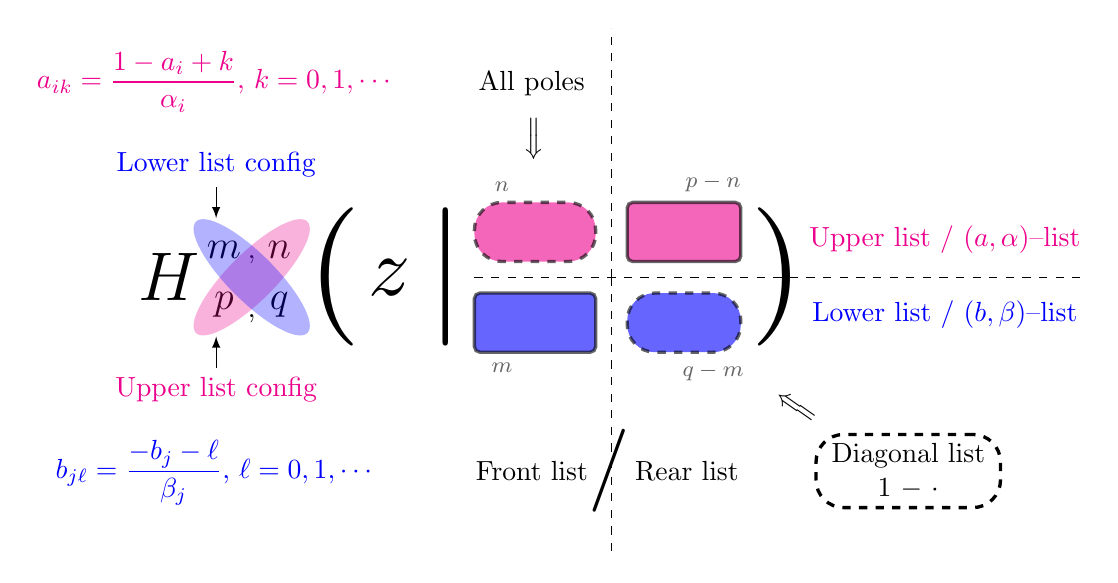
\begin{tikzpicture}[scale=1, transform shape, node distance = 2em, auto]
    \tikzset{>=latex}

    \node (H) at (0,0) {\Huge $H$};
    \node[right of = H, yshift = 1em] (m) {\Large $m$};
    \node[right of = m] (n) {\Large $n$};
    \node[yshift = 0.3em] at ($(m.south)!.5!(n.south)$) {,};

    \node[right of = H, yshift = -1em] (p) {\Large $p$};
    \node[right of = p] (q) {\Large $q$};
    \node[yshift = 0.3em] at ($(p.south)!.5!(q.south)$) {,};

    % Calculate the center coordinate without drawing the path
    \coordinate (center) at ($(n)!0.5!(p)$);

    % Draw the ellipse
    \filldraw[fill = magenta, opacity = 0.3, draw = none, rotate around={-45:(center)}, xshift =0em] (center) ellipse[x radius=0.3, y radius=1];
    \draw[<-] ($(p) + (-0.1,-0.4)$) -- ($(p) + (-0.1,-0.8)$) node [below, color = magenta] (ULC) {Upper list config};

    \filldraw[fill = blue, opacity = 0.3, draw = none, rotate around={+45:(center)}, xshift =0em] (center) ellipse[x radius=0.3, y radius=1];
    \draw[<-] ($(m) + (-0.1,0.4)$) -- ($(m) + (-0.1,0.8)$) node [above, color = blue] (LLC) {Lower list config};

    \node[right of = H, xshift = 4em] (LB) {\scalebox{5}{$($}};
    \node[right of = LB] (z) {\scalebox{3}{$z$}};
    \node[right of = z] (bar) {\scalebox{5}{$|$}};
    \node[right of = bar, xshift = 10 em] (RB) {\scalebox{5}{$)$}};
    \draw [dashed] (bar.east) --++(17em,0) node [above, color = magenta, yshift = 0.5em] {Upper list / $(a,\alpha)$--list} node[below, color = blue, yshift =-0.5em] {Lower list / $(b,\beta)$--list} --++(5em,0);
    \coordinate (ListCenter) at ($(bar)!0.5!(RB)$);
    \draw [dashed] (ListCenter) --++(0, -7em) node [left, xshift = -0.5em] (FrontList) {Front list} node[right, xshift = +0.5em] (RearList) {Rear list} --++(0,-3em);
    \node at ($(RearList)!0.5!(FrontList)$) {\scalebox{3}{$/$}};
    \draw [dashed] (ListCenter) --++(0, +9em);

    \node[right of = RearList, xshift = 6em, rounded corners = 1em, draw, text width = 6em, align=center, very thick, dashed] (DiagList) {Diagonal list\\ $1-\cdot$};
    % \draw [double, -latex, double distance = 4pt] (DiagList.north) --++(-1em, +1em);
    \node[yshift = +1em, xshift = -4em] (Longrightarrow) at (DiagList.north) {\rotatebox[origin=c]{145}{$\Longrightarrow$}};

    \node[yshift = +14em, xshift = -0em] (Poles) at (FrontList) {All poles};
    \node[yshift = -2em] at (Poles) {\rotatebox[origin=c]{-90}{$\Longrightarrow$}};


    \coordinate[yshift = +1em] (UpLstL) at (bar.east);
    \coordinate[yshift = -1em] (LwLstL) at (bar.east);
    \coordinate[yshift = +1em] (UpLstR) at (RB.west);
    \coordinate[yshift = -1em] (LwLstR) at (RB.west);
    \filldraw [fill = magenta, opacity = 0.6, dashed, rounded corners = 1em, very thick] ($(ListCenter) + (-0.2,+0.2)$) rectangle ($(UpLstL) + (0,+0.6)$) node[above, xshift =+1em] {\footnotesize $n$};
    \filldraw [fill = blue,    opacity = 0.6, rounded corners = 0.2em, very thick]       ($(ListCenter) + (-0.2,-0.2)$) rectangle ($(LwLstL) + (0,-0.6)$) node[below, xshift =+1em] {\footnotesize $m$};

    \filldraw [fill = magenta, opacity = 0.6, rounded corners = 0.2em, very thick]       ($(ListCenter) + (+0.2,+0.2)$) rectangle ($(UpLstR) + (0,+0.6)$) node[above, xshift =-1em] {\footnotesize $p-n$};
    \filldraw [fill = blue,    opacity = 0.6, dashed, rounded corners = 1em, very thick] ($(ListCenter) + (+0.2,-0.2)$) rectangle ($(LwLstR) + (0,-0.6)$) node[below, xshift =-1em] {\footnotesize $q-m$};

    \node[yshift = +3em, color = magenta] (pole-a) at (LLC) {$a_{ik} = \dfrac{1-a_i+k}{\alpha_i}$, $k=0,1,\cdots$};
    \node[yshift = -3em, color = blue]    (pole-b) at (ULC) {$b_{j\ell} = \dfrac{-b_j-\ell}{\beta_j}$, $\ell=0,1,\cdots$};
    
  \end{tikzpicture}
\end{document}
